\documentclass[tikz,border=2pt]{standalone}
\usepackage{pgfplots}
\pgfplotsset{compat=1.18}
\begin{document}

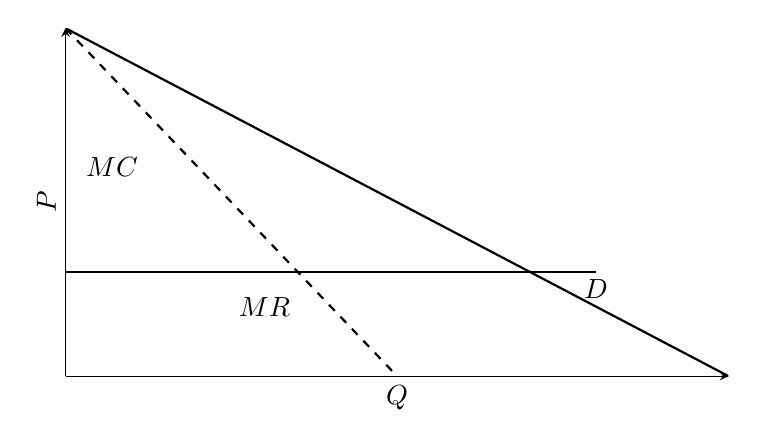
\begin{tikzpicture}
\begin{axis}[
  axis lines=left,
  xlabel={$Q$},
  ylabel={$P$},
  xmin=0, xmax=10,
  ymin=0, ymax=10,
  ticks=none,
  width=10cm,
  height=6cm
]
\addplot[thick, domain=0:10] {10-x};        % Demand
\addplot[thick, dashed, domain=0:5] {10-2*x}; % MR
\addplot[thick, domain=0:8] {3};                         % MC
\node at (axis cs:8,2.5) {$D$};
\node at (axis cs:3,2) {$MR$};
\node at (axis cs:0.7,6) {$MC$};
\end{axis}
\end{tikzpicture}

\end{document}

